% !TEX root = ../thesis.tex

\chapter{Experimental Results}
\mbox{}\\
\mbox{}\\
\mbox{}\\
%TODO add explenation of preciison 
As described in the previous chapter, different strategies were elaborated for both the reward function and the action selection algorithm. Training all possible combinations and then observing the end precision would be a viable way of finding the optimal combination of these. However, due to the training and testing complexities of the algorithms, this would be very time intensive. Instead, we designed a set of experiments with the hope that they would be able to indicate which methods are more optimal.
\subsubsection{Precision measuring}
In order to measure the precision of the result, we observe the fraction of program points at which the Polyhedra invariants generated by our various algorithms is semantically the same as the one generated by ELINA using only online decomposition.
\subsubsection{Training/Testing set}
The algorithms were trained on 328 different benchmarks following the steps mentioned in subsection 4.5. The testing set consists of 81 different benchmarks that were chosen part randomly and part due to their complexity. To avoid overfitting, the testing and training sets do not overlap.


\section{Reward function selection}
As a reminder, if we view the problem as a decision tree and the role of reinforcement learning is to pick the best path at each node, the reward function can be viewed as the compass of the reinforcement learning algorithm that should lead it to the end in such a way as to maximise the global goal.\\
We decided to measure the effectiveness of each reward function by observing if the direction it steered the algorithm to was indeed correctly maximising this global goal. To achieve this, we would first train an algorithm with each of the different reward functions. Once this was done, we modified the Q-learning version of the algorithm so that during testing it would measure each of the different reward functions. As a reminder, the Q-learning algorithm was trained with the following reward function:
\begin{equation}
	r(s_t,a_t,s_{t+1}) = 3  \cdot n_s + 2 \cdot n_b + n_{hb} - \log_{10}(cyc)
\end{equation}
We then ran the Q-learning algorithm measuring each of the new reward functions during the execution. The decision of whether or not the reward function was good was then made with the following rule:\\
If the reward of the deep Q-network algorithm was higher than the one of the Q-learning algorithm, but its overall precision was not higher. This would imply that the deep Q-network was correctly learning to maximise the reward, but that this reward was not maximising the overall results of the algorithm and therefore it was not a good reward.\\
As a reminder, the rewards tested are the following:
 
\begin{equation}
        r_{pr_1}(s_t,a_t,s_{t+1}) = 3  \cdot n_s + 2 \cdot n_b + n_{hb}
\end{equation}
\begin{equation}
        r_{pr_2}(s_t,a_t,s_{t+1}) = 3  \cdot n_s + 2 \cdot n_b + n_{hb} - \log_{10}(|n_b|)
\end{equation}
\begin{equation}
        r_{pr_3}(s_t,a_t,s_{t+1}) = 3  \cdot (n_{s_f} - n_{s_i}) + 2 \cdot (n_{b_f} - n_{b_i}) + (n_{hb_f} - n_{hb_i}) - \log_{10}(|n_b|)
\end{equation}
We obtain the following reward for each join, during the execution of three different benchmarks: 

\begin{figure}[!h]
\minipage{0.32\textwidth}
  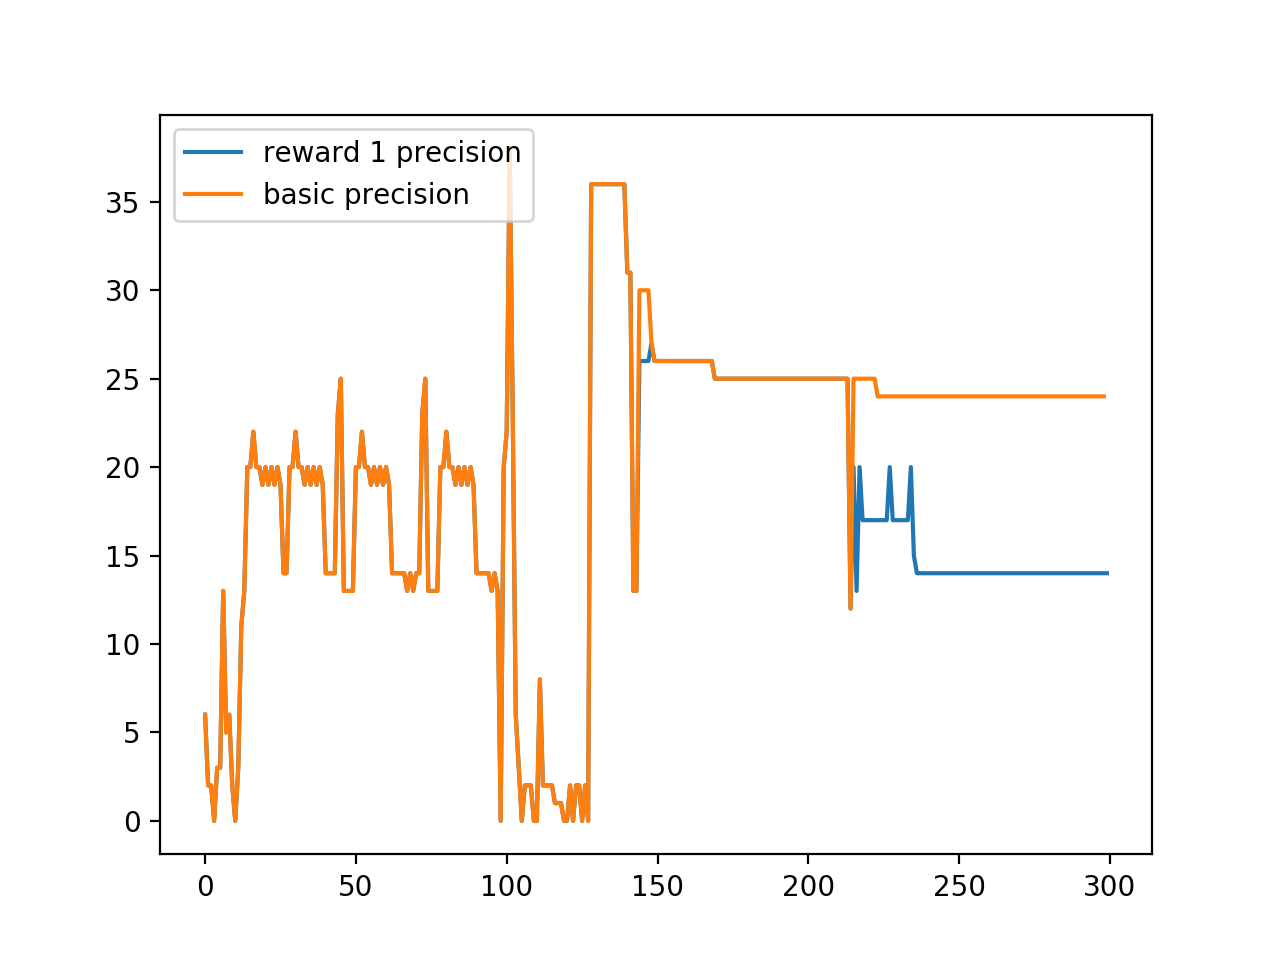
\includegraphics[width=7cm]{figures/r1}
  \caption{Reward one}\label{fig:r1}
\endminipage\hfill
\minipage{0.32\textwidth}
  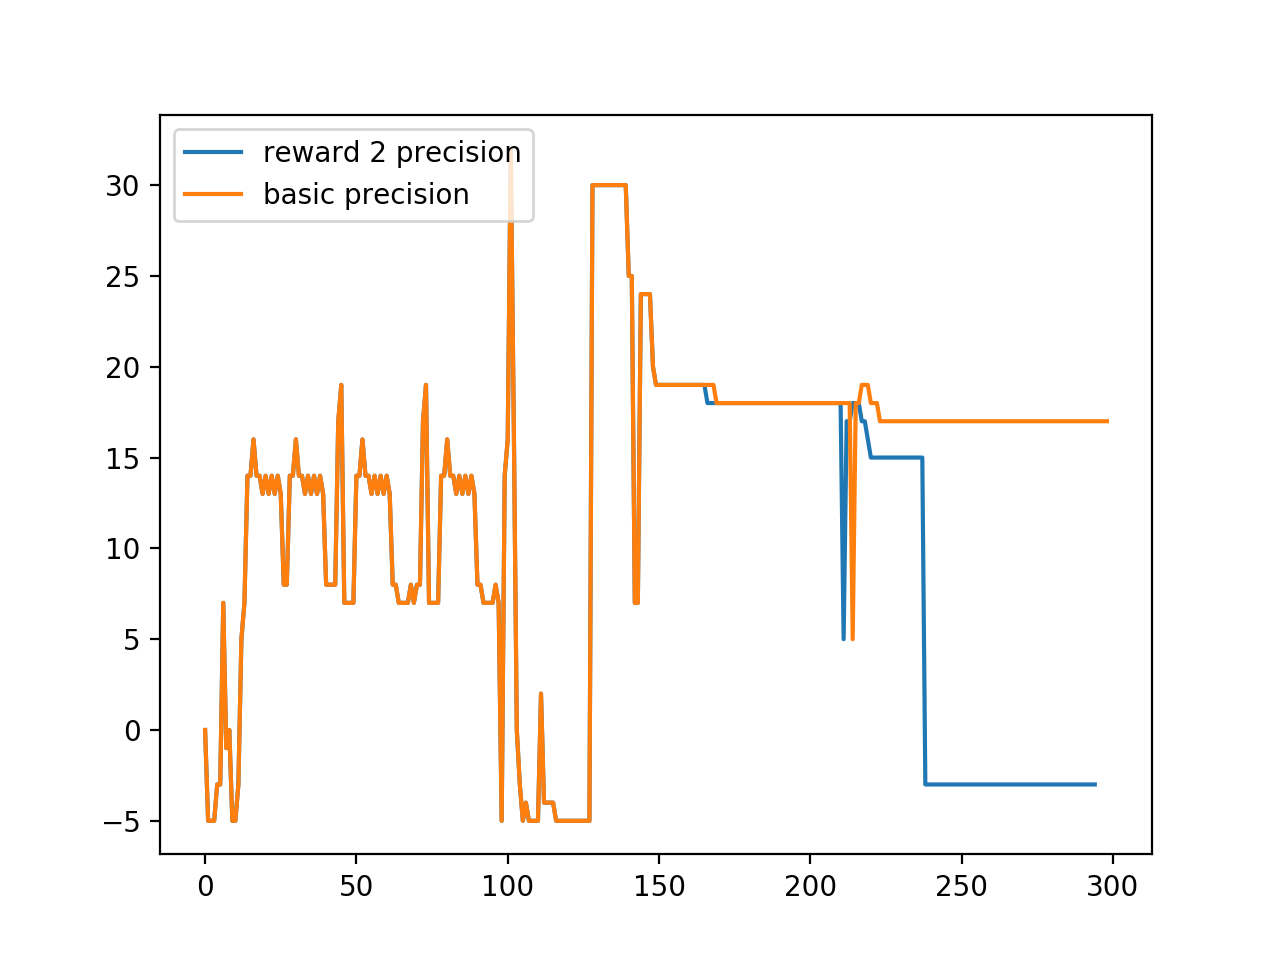
\includegraphics[width=7cm]{figures/r2}
  \caption{Reward two}\label{fig:r2}
\endminipage\hfill
\minipage{0.32\textwidth}%
  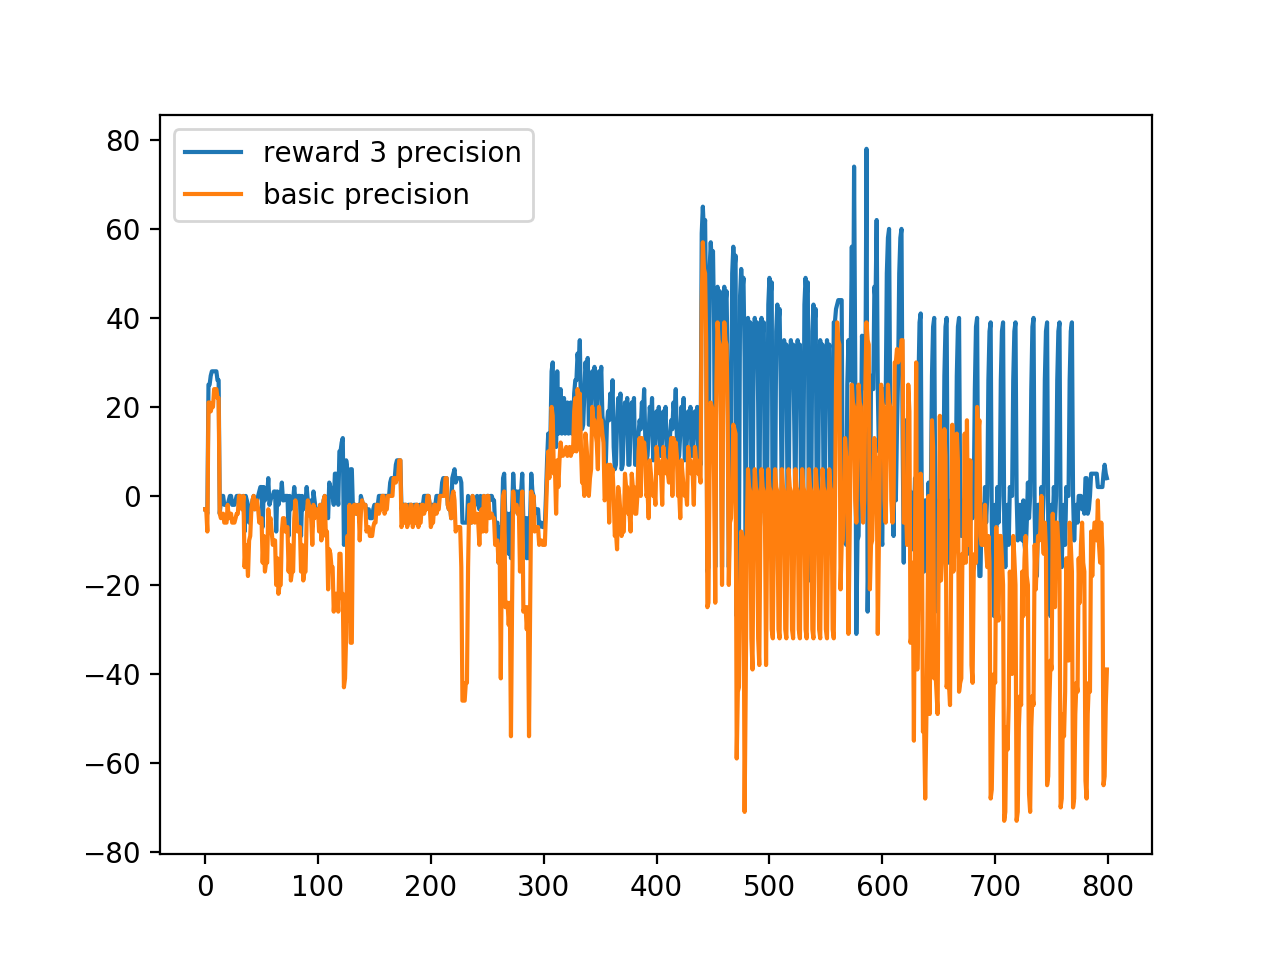
\includegraphics[width=7cm]{figures/r3}
  \caption{Reward three}\label{fig:r3}
\endminipage
\end{figure}

The orange line represents the measured reward whilst running the Q-learning algorithm and the blue line the measured reward of the DQN trained with the corresponding reward. The overall precision of the end polyhedra is the following: For Figure 5.1. 99\% for Q-learning and 96\% for DQN. For figure 5.2. 99\% for Q-learning and 94\% for DQN. For figure 5.3. 97\% for Q-learning and 90\% for DQN. Whilst the graphs behave as expected in the first two scenarios, that is that the reward is lower for the algorithm with lower overall precision as well. In the last graph, we can see something unexpected. Whilst the DQN algorithm has a higher reward throughout most of the execution of the program with an average of 9 versus -8 for the Q-learning algorithm. This indicates that it should also have a better overall precision. However, its overall precision is lower. This tells us that whilst the DQN has learned a correct strategy for maximising the reward, this reward does not guide it to the end goal of maximising the final precision and therefore reward three is not an optimal reward function. These experiments do not give us much information on the differences between reward one and two as they both behave as they should. This is to be expected as reward one and two are similar.\\
It is worth noting that whilst these experiments do give us some interesting information about the effectiveness of the different reward functions, the results are heavily dependant on the benchmark we run them on and therefore the results cannot be fully trusted. However, with the information gathered by these experiments, as well as some overall testing we decided to use the second reward function in further experiments.


\section{Action selection algorithm}
The second problem was selecting the best action selection algorithm. In section 4.3.4., four different action selection algorithms were proposed. In order to select the best one of these, we proceeded by training a DQN using each of them and then comparing the overall precision. Not all the training had to be done separately for the four algorithms. Firstly, we could train estimators from only random actions and then simply specialise each of them with their own action selection algorithm. We then compared the results on a set of seven different benchmarks.
\begin{center}
\captionof{table}{Results of experiments with different action selection algorithms}
\Indm\Indm\Indm\begin{tabular}{||c c c c c c||} 
 
 \hline
 Benchmark & Q-learning & Algorithm 1 & Algorithm 2 & Algorithm 3 & Algorithm 4  \\ [0.5ex] 
 \hline\hline
 driver-media & 99.0 & 98.6 & 97.6 & 93.2 & 98.0 \\ 
 \hline
 linux-kernel-locking-spinlock & 99.9 & 94.4 & 63.6 & 79.9 & 95.0 \\
 \hline
 linux-usb-dev & 58.2 & 51.8 & 60.3 & 56.5 & 59.3\\
 \hline
 linux-kernel-locking-mutex & 77.1 & 73.2 & 95.5 & 95.6 & 76.1\\
 \hline
 complex-emg-drivers-net & 57.1 & 97.3 & 94.6 & 96.0 & 96.9\\ 
 \hline
 complex-emg-drivers-media & 57 & 50.1 & 58.9 & 55.4 & 54.9\\ 
 \hline
 complex-emg-linux-alloc-spinlock & 44.9 & 72.2 & 69.9 & 91.8 & 72.0\\ 
 
 \hline
\end{tabular}
\end{center}

As to the choice of benchmarks for this experiment. We had several criteria. First, we picked benchmarks where achieving a high level of accuracy was not too easy in order to have more informative results. Second, we picked benchmarks that were fast to compute so that the testing time would be fast. We also picked fast benchmarks because the goal was to find an algorithm that maximises the precision as each of these algorithms can be then optimised with their own parameters in order to ameliorate performance and in this way we only had to concentrate on a single goal.\\
As to the results of these experiments. Unfortunately, there is no overall best algorithm. As discussed in section 4.3.4., each of these algorithms has its advantages and shortcomings. However, the main objective we were looking for from these experiments was finding an algorithm that would be stable. We can see that algorithms two and three can obtain very good results on some benchmarks. Unfortunately, their performance is far from optimal on others. This is due to the fact that both of these are strongly threshold dependant and picking an optimal threshold that would work well for all benchmarks is very difficult, making both of these algorithms not practical. Afterwards, between the first and fourth algorithm, the last one outperforms the first on average and therefore is the one we will use from here on. Whilst the last algorithm does not have the best precision on some benchmarks, its stability overall benchmarks made it the preferred candidate.


\section{Final algorithm}
Once both decisions were made, the architecture of the final separated algorithm was fully decided and could, therefore, be further trained and optimised.\\
For the testing of the different algorithms, we decided to run them on a large set of benchmarks. In this way, we could see if they managed to learn a global policy or simply find local minima. In the end, we settled on a set of 81 different benchmarks of varying sizes and complexities. Due to the relatively large number of benchmarks, we set the timeout to be quite short, more specifically thirty minutes. This was done so that the experiments could be run in a reasonable amount of time. For each benchmark, we saved the resulting invariants of the analysis and the runtime.\\
\mbox{}\\
We test the benchmarks using four different analyses:
\begin{itemize}
    \item Using the decomposed Polyhedra domain, to have a baseline for precision.
    \item RL trained with Q-learning
    \item Basic deep Q-network algorithm
    \item Deep Q-network with separated estimators
\end{itemize}

The following table displays the results of the experiments. It shows the average of the precision percentages when compared to the abstraction-less analysis. The total runtime on all benchmarks, the number of benchmarks that the analysis timed out on. The number of benchmarks where the algorithm achieved $100\%$ precision. Finally, for the reinforcement learning algorithms, the number of benchmarks where they outperform the other RL algorithms with regards to precision. 

\begin{center}
\captionof{table}{Results with final algorithms}
\begin{tabular}{||c c c c c||}
 
 \hline
 Results on 81 bench. & Elina & Q-learning & DQN & Separated DQN \\ [0.5ex] 
 \hline\hline
 Avg. prec. (\%) & 100 & 87.1 & 94.9 & 91.6\\
 Runtime (hr.) & 18:28 & 14:05 & 15:35 & 11:21\\
 $n^{\circ}$ timeouts & 33 & 23 & 23 & 17\\
 $n^{\circ}$ bench. 100\% prec. & 81 & 13 & 27 & 18\\
 $n^{\circ}$ bench. most precise &  & 1 & 36 & 2\\
 
 \hline
\end{tabular}
\end{center}

\subsubsection{Result discussion}
As shown in the results, we were able to outperform the Q-learning method with both the deep Q-network and the separated deep Q-network algorithms with regards to accuracy. What is interesting to note, is that the regular DQN outperforms the separated one in terms of precision. This can most likely be explained by the action selection algorithm. Even though in 5.2., we attempted to pick an algorithm that would be as stable as possible and be able to maintain good results overall benchmarks. The results show that on a few benchmarks the separated DQN performs very poorly, thus reducing its overall precision. However, it is worth noting that the separated DQN outperforms all the other algorithms in terms of performance, as it manages to finish the analysis of all the benchmarks quite a lot faster than the others, most notably, it is faster than the Q-learning algorithm whilst remaining more precise as well. The separated DQN also has the least timeouts out of all the analyses. In terms of precision, however, the normal DQN algorithm is the most precise on average overall benchmarks. It is also more precise on 36 of the 81 benchmarks and is only beaten on one benchmark by Q-learning and on two by the separated DQN, the precision remains the same on the rest. It also achieves $100\%$ precision on more than double the number of benchmarks than the Q-learning method does.  
































